% !TEX root = main.tex
\begin{subsection}{A Partial Upper Bound}\label{sec:IntroMainThm}
In this section, we show how to compute an upper bound on $\rho$, with a user-defined confidence $\beta \in [0, 1)$. We do this by constructing a $l$-step CQLF which is valid with probability at least $\beta$. Note that, the existence of a $l$-step CQLF implies 
$\rho \leq \gamma^*$ due to Theorem \ref{thm:cqlf}. Even though to find this CQLF in practice, one would solve the feasibility problem on $P$ induced by problem \eqref{eq:lowerbound} once $\gamma^*$ is found, for the sake of rigor and clarity of our proofs, we introduce a slighly different optimization problem. We consider the following optimization problem, referred by $\Opt(\omega_N)$ for the rest of the discussion:
\begin{equation}\label{eqn:campiOpt03}
\begin{aligned}
& \min_{P} & & \lambda_{\max}(P) \\
& \text{s.t.} 
&  & (\mathbf{A}x)^T P \mathbf{A} x \leq { \left( (1 +\eta)\gamma^*(\omega_N) \right)}^{2l} x^T P x,\\
& && \qquad \qquad \qquad \qquad \qquad \forall\ (x, \mathbf{j}) \in \omega_N \\
& && P \succeq I, \\
\end{aligned}
\end{equation}
with $\eta > 0$, and $\gamma^*(\omega_N)$ the optimal solution to the optimization problem \eqref{eq:lowerbound}. Let us analyze the relationship between $\Opt(\omega_N)$ and the optimization problem \eqref{eq:lowerbound}. Firstly, thanks to the homogeneity of the system, we can replace the constraint $P \succ 0$ in the initial problem with the constraint $P \succeq I$. Secondly, for reasons that will become clear later in the discussion, we want to take the objective function as $\lambda_{\max}(P)$ (which is convex), instead of solving a feasibility problem in $P$. Lastly, we introduced a ``regularization parameter'', $\eta > 0$, which ensures strict feasibility of $\Opt(\omega_N)$. As the reader will see, we will derive results valid for arbitrarily small values of $\eta$. This will then not hamper the practical accuracy of our technique, while allowing us to derive a theoretical asymptotic guarantee (i.e., for large number of observations). From now, we denote the optimal solution of $\Opt(\omega_N)$ by $P(\omega_N)$, and drop the explicit dependence of $P$ on $\omega_N$ when it is clear from the context.

The curious question whether the optimal solution of this sampled problem is a feasible solution to \eqref{eqn:campiOpt2} has been widely studied in the literature \cite{campi}. It turns out that under certain technical assumptions, one can bound the proportion of the constraints of the original problem \eqref{eqn:campiOpt2} that are violated by the optimal solution of $\Opt(\omega_N)$, with some probability which is a function of the sample size $N$. In the following theorem, we adapt a classical result from random convex optimization literature to our problem.
\begin{thm}[adapted from Theorem 3.3\footnotemark, \cite{campi}]\label{mainTheorem0}
Let $d$ be the dimension of $\Opt(\omega_N)$ and $N \geq d+1$. Consider the optimization problem $\Opt(\omega_N)$ given in \eqref{eqn:campiOpt03}, where $\omega_N$ is a uniform random sample drawn from the set $Z_l$.
Then, for all $\varepsilon \in (0,1]$ the following holds:
\begin{equation}\label{eqn:violation}
\mu_l^N\hspace{-1mm}\left\{ \omega_N \in Z_l^N: \mu_l \left( V(\omega_N) \right) \leq \varepsilon \right\}\hspace{-1mm} \geq \beta(\varepsilon, N),
\end{equation}
where $\mu_l^N$ denotes the product probability measure on $Z_l^N$, $\beta(\varepsilon, N) =  1- \sum_{j=0}^{d} \binom{N}{j}\varepsilon^j (1-\varepsilon)^{N-j}$, and $V(\omega_N)$ is the set $\{(x,\mathbf{j}) \in Z_l: (\mathbb{A}_l x)^T P(\omega_N) \mathbb{A}_l x > (\gamma_{\omega_N}^{*})^{2l} x^T P(\omega_N) x\}$, i.e., it is the set of constraints that are violated by the optimal solution of $\Opt(\omega_N)$.
\end{thm}

\footnotetext{Theorem 3.3 in \cite{campi} requires $\Opt(\omega_N)$ to satisfy the following technical assumptions:\begin{enumerate}
\item When the problem $\Opt(\omega_N)$ admits an optimal solution, this solution is unique.
\item Problem $\Opt(\omega_N)$ is nondegenerate with probability $1$.
\end{enumerate}
Here, the first assumption can be enforced if required by adding a tie-breaking rule to $\Opt(\omega_N)$ as explained in Appendix A in \cite{tiebreak}, while the second assumption can be lifted, as explained in PART 2b in \cite{campi-garatti}, thanks to the introduction of a ``constraint heating''.
}

\begin{cor}\label{cor:gettingRidOfm}
Consider a set of matrices $\mathcal{M}$, $\gamma^{*}$ optimal solution of \eqref{eq:lowerbound} and matrix $P \succ 0$ optimal solution of $\Opt(\omega_N)$. Then $P$ satisfies: 
\begin{equation}\label{eqn:P0}
(\mathbf{A}_l x)^T P \mathbf{A}_l x \leq (\gamma^{*})^{2l} x^T P x, \forall x \in \sphere \setminus \tilde{\sphere}, \forall \mathbf{j} \in M^l
\end{equation} 
with $\tilde{\sphere} = \pi_\sphere(V(\omega_N)) \subset \sphere$ such that $\sigma^{n-1}(\tilde{\sphere}) \leq \varepsilon m^l $.
\end{cor}

The proof of Corollary~\ref{cor:gettingRidOfm} is based on straightforward arguments on measures, and is given in \textcolor{red}{[technical report]}. This result allows us to only consider set of violating points on the sphere from now. Note that, this result is conservative: the case where we have the equality $\sigma(\tilde{\sphere}) = \varepsilon m^l$ corresponds to the case where we have only observed one mode for the entirety of the trace and have then minimal knowledge on the system for a given $\varepsilon$.


The above results allow us to conclude, from a finite number of observations, that with probability $\beta$ (where $\beta$ goes to $1$ as $N$ goes to infinity), the required property is actually satisfied for the complete sphere $\sphere$, except on a small set of measure at most $\tilde{\varepsilon} = \varepsilon m^l$. This means that, the ellipsoid $E_P$ computed by $\Opt(\omega_N)$ is ``almost invariant"  except on a set of measure bounded by $\tilde{\varepsilon}$. This can be represented in the case $n=2$ by the following plot, where the red points of $E_P$ are points that might violate the contractivity constraint. Here, the set of red points has measure at most $\tilde{\varepsilon}$.
\begin{figure}[H]\label{fig:ellipsoid}
\begin{center}
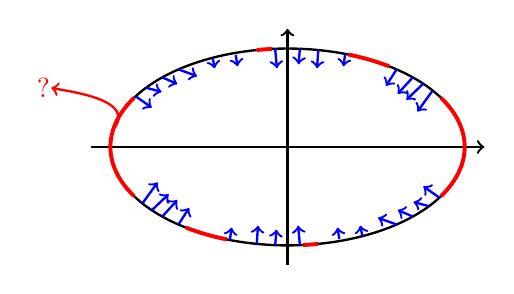
\begin{tikzpicture}[scale=0.5]
\draw[line width=0.3mm,black,->] (-5,0) -- (5,0);
\draw[line width=0.3mm,black,->] (0,-3) -- (0,3);

\draw [line width = 0.5mm,red,domain=-30:30] plot ({4.5 * cos(\x)}, {2.5 * sin(\x)});
\draw [line width = 0.3mm,black,domain=30:55] plot ({4.5 * cos(\x)}, {2.5 * sin(\x)});
\draw [line width = 0.5mm,red,domain=55:70] plot ({4.5 * cos(\x)}, {2.5 * sin(\x)});
\draw [line width = 0.3mm,black,domain=70:95] plot ({4.5 * cos(\x)}, {2.5 * sin(\x)});
\draw [line width = 0.5mm,red,domain=95:100] plot ({4.5 * cos(\x)}, {2.5 * sin(\x)});
\draw [line width = 0.3mm,black,domain=100:150] plot ({4.5 * cos(\x)}, {2.5 * sin(\x)});
\draw [line width = 0.5mm,red,domain=150:210] plot ({4.5 * cos(\x)}, {2.5 * sin(\x)});
\draw [line width = 0.3mm,black,domain=210:235] plot ({4.5 * cos(\x)}, {2.5 * sin(\x)});
\draw [line width = 0.5mm,red,domain=235:250] plot ({4.5 * cos(\x)}, {2.5 * sin(\x)});
\draw [line width = 0.3mm,black,domain=250:275] plot ({4.5 * cos(\x)}, {2.5 * sin(\x)});
\draw [line width = 0.5mm,red,domain=275:280] plot ({4.5 * cos(\x)}, {2.5 * sin(\x)});
\draw [line width = 0.3mm,black,domain=280:330] plot ({4.5 * cos(\x)}, {2.5 * sin(\x)});

\draw[->,line width=0.3mm,red] (-4.432,0.434) .. controls (-3.8,1.2) and (-5.5,1.4) .. (-6,1.5);
\draw[red] (-6.2,1.5) node {?};

\draw[->,line width = 0.3mm,blue] (3.6862,1.4339) -- (3.3,0.9);
\draw[->,line width = 0.3mm,blue] (3.4472,1.6070) -- (3.02,1.2);
\draw[->,line width = 0.3mm,blue] (3.182,1.7678) -- (2.8,1.35);
\draw[->,line width = 0.3mm,blue] (2.7705,1.97) -- (2.5,1.55);
\draw[->,line width = 0.3mm,blue] (-3.6862,-1.4339) -- (-3.3,-0.9);
\draw[->,line width = 0.3mm,blue] (-3.4472,-1.6070) -- (-3.02,-1.2);
\draw[->,line width = 0.3mm,blue] (-3.182,-1.7678) -- (-2.8,-1.35);
\draw[->,line width = 0.3mm,blue] (-2.7705,-1.97) -- (-2.5,-1.55);
\draw[->,line width = 0.3mm,blue] (1.4651,2.3638) -- (1.42,2.05);
\draw[->,line width = 0.3mm,blue] (0.7814,2.4620) -- (0.75,2);
\draw[->,line width = 0.3mm,blue] (0.3139,2.4939) -- (0.28,2.1);
\draw[->,line width = 0.3mm,blue] (-0.3139,2.4939) -- (-0.27,2);      
\draw[->,line width = 0.3mm,blue] (-1.4651,-2.3638) -- (-1.42,-2.05);
\draw[->,line width = 0.3mm,blue] (-0.7814,-2.4620) -- (-0.75,-2);
\draw[->,line width = 0.3mm,blue] (-0.3139,-2.4939) -- (-0.28,-2.1);
\draw[->,line width = 0.3mm,blue] (0.3139,-2.4939) -- (0.27,-2);
\draw[->,line width = 0.3mm,blue] (-1.3157,2.33908) -- (-1.27,2.05);
\draw[->,line width = 0.3mm,blue] (-1.9018,2.2658) -- (-1.85,2);
\draw[->,line width = 0.3mm,blue] (-2.7705,1.97) -- (-2.3,1.8);
\draw[->,line width = 0.3mm,blue] (-3.182,1.7678) -- (-2.8,1.6);      
\draw[->,line width = 0.3mm,blue] (-3.5939,1.5045) -- (-3.2,1.4); 
\draw[->,line width = 0.3mm,blue] (-3.8573,1.2876) -- (-3.45,1); 
\draw[->,line width = 0.3mm,blue] (1.3157,-2.33908) -- (1.27,-2.05);
\draw[->,line width = 0.3mm,blue] (1.9018,-2.2658) -- (1.85,-2);
\draw[->,line width = 0.3mm,blue] (2.7705,-1.97) -- (2.3,-1.8);
\draw[->,line width = 0.3mm,blue] (3.182,-1.7678) -- (2.8,-1.6);      
\draw[->,line width = 0.3mm,blue] (3.5939,-1.5045) -- (3.2,-1.4); 
\draw[->,line width = 0.3mm,blue] (3.8573,-1.2876) -- (3.45,-1); 
\end{tikzpicture}
\end{center}
\caption{Representation of the ``partial invariance property'' obtained by application of the results in Theorem~\ref{mainTheorem0}. A priori, we know nothing about the images of the red points. Our goal is to convert this partial invariance property into a global stability property.}
\end{figure}
\vspace{-0.5cm}
Thus, we are left with the following question: 
\vspace{-0.2cm}
\begin{prob}\label{prob:question}
What can we conclude on the JSR if the Lyapunov property is satisfied by all points, except a set of measure $\tilde{\varepsilon}$?
\end{prob}
We will answer to this question by considering the largest ellipsoid included in the convex hull of the points of $E_P$ that satisfy the invariance property. This ellipsoid will indeed satisfy our invariance property thanks to the following key property of switched linear systems.

\begin{property}\label{property:convpres}
The dynamics given in \eqref{eq:switchedSystem} is convexity-preserving, meaning that for any set of points $X \subset \mathbb{R}^n$, we have $f(\conv({X})) \subset \conv(f(X))$.
\end{property}

Of course, for a fixed measure $\tilde{\varepsilon}$, this largest ellipsoid will depend on the distribution of points of $E_P$ that violate the constraint. In order to obtain a guarantee on our upper bound, we will look for the smallest such ellipsoid obtained over all possible sets $V(\omega_N)$ of measure $\tilde{\varepsilon}$. In the particular case where $E_P = \sphere$, we benefit of the following tool.
\begin{defn}
We define the \emph{spherical cap} on $\sphere$ for a given hyperplane $c^Tx = k$ as $\mathcal{C}_{c,k} := \{x \in \sphere : c^Tx >k\}$.
\end{defn}
We now define the function 
\begin{equation}\label{shrinkage}
\Delta: \left\{
    \begin{split}
    &\wp(\sphere) \to [0,1]\\ 
    &X \mapsto \sup \{r: r\ball \subset \conv(\sphere \setminus X)\}.
    \end{split}
  \right.
\end{equation}
The following proposition tells us that $\Delta$ is minized when $X$ is a spherical cap, i.e., the minimal radius $\delta$ of the largest sphere $\delta \sphere$ included in $\sphere \setminus X$ will be reached when $X$ is a spherical cap.
\begin{prop}\label{thm:mainSphericalCap}
Let $\mathcal{X}_{\tilde{\varepsilon}} = \{X \subset \sphere: \sigma^{n-1}(X) \leq \tilde{\varepsilon}\}$. Then, for any $\tilde{\varepsilon} \in [0,1]$, the function $\Delta(X)$ attains its minimum over $\mathcal{X}_{\tilde{\varepsilon}}$ for some $X$ which is a spherical cap.
\end{prop}
A proof of Proposition~\ref{thm:mainSphericalCap} is given in \textcolor{red}{technical report}. By homogeneity of the system, we have $x \in \tilde{\sphere} \iff -x \in \tilde{\sphere}$, which implies that the minimal $\delta$ will in fact occur when the set of violating points is the union of two symmetric spherical caps, each of measure $\frac{\tilde{\varepsilon}}{2}$.

\begin{figure}[H]
\begin{center}
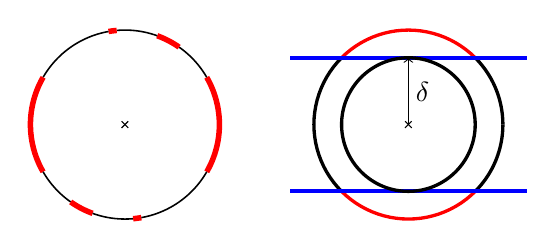
\begin{tikzpicture}[scale=0.6]
\draw (0.07,-0.07) -- (-0.07,0.07);
\draw (0.07,0.07) -- (-0.07,-0.07);
\draw[line width = 0.7mm,red,domain=-30:30] plot ({2*cos(\x)}, {2*sin(\x)});
\draw[line width = 0.2mm,black,domain=30:55] plot ({2 * cos(\x)}, {2 * sin(\x)});
\draw[line width = 0.7mm,red,domain=55:70] plot ({2 * cos(\x)}, {2 * sin(\x)});
\draw[line width = 0.2mm,black,domain=70:95] plot ({2 * cos(\x)}, {2 * sin(\x)});
\draw[line width = 0.7mm,red,domain=95:100] plot ({2 * cos(\x)}, {2 * sin(\x)});
\draw[line width = 0.2mm,black,domain=100:150] plot ({2 * cos(\x)}, {2 * sin(\x)});
\draw[line width = 0.7mm,red,domain=150:210] plot ({2 * cos(\x)}, {2 * sin(\x)});
\draw[line width = 0.2mm,black,domain=210:235] plot ({2 * cos(\x)}, {2 * sin(\x)});
\draw[line width = 0.7mm,red,domain=235:250] plot ({2 * cos(\x)}, {2 * sin(\x)});
\draw[line width = 0.2mm,black,domain=250:275] plot ({2 * cos(\x)}, {2 * sin(\x)});
\draw[line width = 0.7mm,red,domain=275:280] plot ({2 * cos(\x)}, {2 * sin(\x)});
\draw[line width = 0.2mm,black,domain=280:330] plot ({2 * cos(\x)}, {2 * sin(\x)});

\draw (5.93,-0.07) -- (6.07,0.07);
\draw (5.93,0.07) -- (6.07,-0.07);
\draw [black,very thick,domain=0:45] plot ({6+2*cos(\x)}, {2*sin(\x)});
\draw [red,very thick,domain=45:135] plot ({6+2*cos(\x)}, {2*sin(\x)});
\draw [black,very thick,domain=135:225] plot ({6+2*cos(\x)}, {2*sin(\x)});
\draw [red,very thick,domain=225:315] plot ({6+2*cos(\x)}, {2*sin(\x)});
\draw [black,very thick,domain=315:360] plot ({6+2*cos(\x)}, {2*sin(\x)});
\draw[line width = 0.5mm,blue] (3.5,1.414) -- (8.5,1.414);
\draw[line width = 0.5mm,blue] (3.5,-1.414) -- (8.5,-1.414);
\draw[->] (6,0) -- (6,1.414);
\draw (6.3,0.7) node {$\delta$};
\draw [black,very thick] (6,0) circle [radius = 1.414cm];
\end{tikzpicture}
\end{center}
\caption{On the left, case when the ellipse in Fig.~\ref{fig:ellipsoid} is a sphere. On the right, case giving minimal $\delta$. The set of points violating the invariance constraint (in red) is the union of two spherical caps, each of measure $\tilde{\varepsilon}$.}
\end{figure}

\begin{rem}
When $\varepsilon \geq \frac{1}{m^l}$, we have $\tilde{\varepsilon} \geq 1$ and $\delta(\tilde{\varepsilon}) = 0$: the upper we can give for the JSR is then only $+ \infty$.
\end{rem}
\end{subsection}


\begin{subsection}{A global upper bound}
In this section, we give an answer to Problem~\ref{prob:question} in Theorem~\ref{thm:mainTheorem01}. In order to use the properties for spheres given in the previous section, we will have to relate $E_{P(\omega_N)}$ to $\sphere$. In order to do thi, we apply a change of coordinates bringing $E_P$ to $\sphere$. Since $P \in \mathcal{S}_{++}^n$, it can be written in its Cholesky form 
\begin{equation}\label{cholesky}
P = L^TL,
\end{equation} 
where $L$ is an upper triangular matrix. Note that, $L$ maps the elements of $E_P$ to $\sphere$.
\begin{figure}[H]
\begin{center}
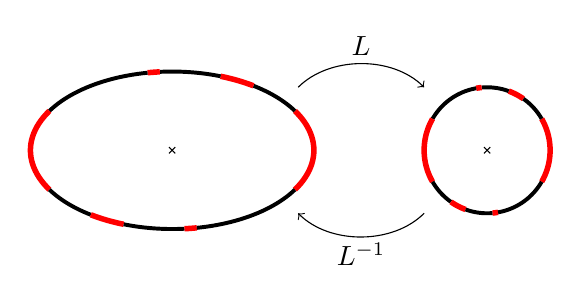
\begin{tikzpicture}[scale=0.4]
\draw (-4-0.1,-0.1) -- (-4+0.1,0.1);
\draw (-4-0.1,0.1) -- (-4+0.1,-0.1);
\draw [line width = 0.7mm,red,domain=-30:30] plot ({-4 + 4.5 * cos(\x)}, {2.5 * sin(\x)});
\draw [line width = 0.5mm,black,domain=30:55] plot ({-4 + 4.5 * cos(\x)}, {2.5 * sin(\x)});
\draw [line width = 0.7mm,red,domain=55:70] plot ({-4 + 4.5 * cos(\x)}, {2.5 * sin(\x)});
\draw [line width = 0.5mm,black,domain=70:95] plot ({-4 + 4.5 * cos(\x)}, {2.5 * sin(\x)});
\draw [line width = 0.7mm,red,domain=95:100] plot ({-4 + 4.5 * cos(\x)}, {2.5 * sin(\x)});
\draw [line width = 0.5mm,black,domain=100:150] plot ({-4 + 4.5 * cos(\x)}, {2.5 * sin(\x)});
\draw [line width = 0.7mm,red,domain=150:210] plot ({-4 + 4.5 * cos(\x)}, {2.5 * sin(\x)});
\draw [line width = 0.5mm,black,domain=210:235] plot ({-4 + 4.5 * cos(\x)}, {2.5 * sin(\x)});
\draw [line width = 0.7mm,red,domain=235:250] plot ({-4 + 4.5 * cos(\x)}, {2.5 * sin(\x)});
\draw [line width = 0.5mm,black,domain=250:275] plot ({-4 + 4.5 * cos(\x)}, {2.5 * sin(\x)});
\draw [line width = 0.7mm,red,domain=275:280] plot ({-4 + 4.5 * cos(\x)}, {2.5 * sin(\x)});
\draw [line width = 0.5mm,black,domain=280:330] plot ({-4 + 4.5 * cos(\x)}, {2.5 * sin(\x)});

\draw (5.9,-0.1) -- (6.1,0.1);
\draw (5.9,0.1) -- (6.1,-0.1);
\draw [line width = 0.7mm,red,domain=-30:30] plot ({6 + 2 * cos(\x)}, {2 * sin(\x)});
\draw [line width = 0.5mm,black,domain=30:55] plot ({6 + 2 * cos(\x)}, {2 * sin(\x)});
\draw [line width = 0.7mm,red,domain=55:70] plot ({6 + 2 * cos(\x)}, {2 * sin(\x)});
\draw [line width = 0.5mm,black,domain=70:95] plot ({6 + 2 * cos(\x)}, {2 * sin(\x)});
\draw [line width = 0.7mm,red,domain=95:100] plot ({6 + 2 * cos(\x)}, {2 * sin(\x)});
\draw [line width = 0.5mm,black,domain=100:150] plot ({6 + 2 * cos(\x)}, {2 * sin(\x)});
\draw [line width = 0.7mm,red,domain=150:210] plot ({6 + 2 * cos(\x)}, {2 * sin(\x)});
\draw [line width = 0.5mm,black,domain=210:235] plot ({6 + 2 * cos(\x)}, {2 * sin(\x)});
\draw [line width = 0.7mm,red,domain=235:250] plot ({6 + 2 * cos(\x)}, {2 * sin(\x)});
\draw [line width = 0.5mm,black,domain=250:275] plot ({6 + 2 * cos(\x)}, {2 * sin(\x)});
\draw [line width = 0.7mm,red,domain=275:280] plot ({6 + 2 * cos(\x)}, {2 * sin(\x)});
\draw [line width = 0.5mm,black,domain=280:330] plot ({6 + 2 * cos(\x)}, {2 * sin(\x)});
\draw[->] (0,2) .. controls (1,3) and (3,3) .. (4,2);
\draw[->] (4,-2) .. controls (3,-3) and (1,-3) .. (0,-2); 
\draw (2,3.3) node {$L$};
\draw (2,-3.3) node {$L^{-1}$};
\end{tikzpicture}
\end{center}
\caption{Change of coordinates to bring our problem back to the case of the unit sphere.}
\end{figure}
%We now know how to compute an upper bound on the JSR when the ``almost invariant" ellipsoid is $\sphere$. Thanks to Property \ref{rem:scaling}, if this is not the case, we can simply perform a change of coordinates mapping this ellipsoid to $\sphere$ and compute the JSR in the new coordinates system instead. To do this, in the next theorem, we bound the measure of violating constraints on $\sphere$ after the change of coordinates, in terms of the measure of the violated constraints on $\sphere \times M^l$ in the original coordinates.
\begin{thm}\label{thm:mainTheorem01}
Let $\gamma^* \in \mathbb{R}_{> 0}$. Consider a set of matrices $\mathcal{M}$, and a matrix $P \succ 0$ optimal solution of \eqref{eqn:P0} for some $\tilde{\sphere} \subset \sphere$ where $\sigma^{n-1}(\tilde{\sphere}) \leq \tilde{\varepsilon}$. Then, we have $$\rho(\mathcal{M}) \leq \frac{\gamma^{*}}{\sqrt[l]{\delta \left( \frac{\tilde{\varepsilon} \kappa(P)}{2} \right)}}$$ with $\kappa(P) = \sqrt{\frac{\lambda_{\max}(P)^n}{\det(P)}}$ and $\delta(x) = \sqrt{1- I^{-1} \left(2 x; \frac{n-1}{2}, \frac{1}{2} \right)}$ ($I$ is the regularized incomplete beta function). 
\end{thm}

\begin{pf*}{Proof.}
\textit{i)} Since we have seen in the previous section a technique to solve the spherical case, we first bring our problem to the spherical case. To do so, we perform the change of coordinates defined as in \eqref{cholesky} by $L \in \mathcal{L}(\mathbb{R}^n)$ which maps the ellipsoid $E_P$ to the sphere $\sphere$. By defining \mbox{$\bar{A}_{j_i}=  L A_{j_i} L^{-1}$,} and $\barAl = \bar{A}_{j_l} \bar{A}_{j_{l-1}} \dots \bar{A}_{j_1} $, problem \eqref{eqn:P0} becomes:
\begin{equation}\label{eq:assumption3}
(\bar{\mathbf{A}}_l x)^T \bar{\mathbf{A}}_l x \leq ({\gamma^*})^{2l} x^T x, \, \forall x \in L^{-1}(\sphere \setminus \tilde{\sphere}), \forall \mathbf{j} \in M^l.
\end{equation}
By using the homogeneity of the dynamics, we have:
\begin{equation*}
\begin{aligned}
&(\bar{\mathbf{A}}_l x)^T \bar{\mathbf{A}}_l x \leq ({\gamma^*})^{2l} x^T x,\, \forall x \in L^{-1}(\sphere \setminus \tilde{\sphere}) \\ &\quad \implies (\bar{\mathbf{A}}_l x)^T \bar{\mathbf{A}}_l x \leq ({\gamma^*})^{2l} x^T x,\, \forall x \in \Pi_\sphere \left( L^{-1}(\sphere \setminus \tilde{\sphere}) \right),
\end{aligned}
\end{equation*}
and therefore we can rewrite \eqref{eq:assumption3} as:
\begin{equation}\label{eq:assumption4}
(\bar{\mathbf{A}}_l x)^T \bar{\mathbf{A}}_l x \leq ({\gamma^*})^{2l} x^T x, \forall x \in \sphere \setminus \Pi_\sphere(L^{-1}\tilde{\sphere}), \forall \mathbf{j} \in M^l.
\end{equation}

\textit{ii)} We now show how to relate $\sigma^{n-1}(\proj_\sphere(L^{-1}(\tilde{\sphere})))$ to $\sigma^{n-1}(\tilde{\sphere})$, measure of the violating set in the initial coordinates. Consider $\sphere^{\tilde{\sphere}}$, the sector of $\ball$ defined by $\tilde{\sphere}$. We denote $C:= L^{-1}(\tilde{\sphere})$ and $C':=\proj_\sphere(L^{-1}(\tilde{\sphere}))$. We have $\proj_{\sphere}(C) = C'$ and $\sphere^{C'} \subset \frac{1}{ \lambda_{\min (L^{-1})}} C$. This leads to:
$$\sigma^{n-1}(C') = \lambda \left( \sphere^{C'} \right) \leq \lambda \left( \frac{1}{ \lambda_{\min (L^{-1})}} E_{P'}^{C} \right).$$ Then, the following holds: 
\begin{eqnarray}
\nonumber\sigma^{n-1}(C') \leq \frac{\lambda(E_{P'}^{C})}{\lambda_{\min}(L^{-1})^n} &\leq& \frac{\lambda \left( L^{-1}(\sphere^{\tilde{\sphere}}) \right)}{\lambda_{\min}(L^{-1})^n} \\
\label{eqn:lt} &=&\frac{|\det(L^{-1})|}{\lambda_{\min}(L^{-1})^n}\lambda \left( \sphere^{\tilde{\sphere}} \right) \\
\label{eqn:map1} &=&\sqrt{\frac{\lambda_{\max}(P)^n}{\det(P)}}\sigma^{n-1}(\tilde{\sphere})
\end{eqnarray}
where \eqref{eqn:lt} follows from the fact that $\lambda(Q(X)) = |\det(Q)| \lambda(X)$, for any set $X \subset \mathbb{R}^n$ and $Q \in \mathcal{L}(\mathbb{R}^n)$ (see e.g. \cite{rudin}). Hence, we have
\begin{equation}\label{eqn:contraction}
(\bar{\mathbf{A}}_l x)^T \bar{\mathbf{A}}_l x \leq (\gamma^{*})^{2l} x^Tx, \forall x \in \sphere \setminus \sphere', \forall \mathbf{j} \in M^l,
\end{equation}
with $\sphere' = \Pi_\sphere(L^{-1}\tilde{\sphere})$ and $\sigma^{n-1}(\sphere') = \sqrt{\frac{\lambda_{\max}(P)^n}{\det(P)}}\sigma^{n-1}(\tilde{\sphere})= \kappa(P) \tilde{\varepsilon}$.


\textit{iii)} For a such given set $\sphere'$, we look for the largest sphere included in $\convhull (\sphere \setminus \sphere')$. By homogeneity of the system, this sphere is centered at the origin, and we denote by $\alpha$ its radius. By \eqref{eqn:contraction}, $l$-traces initialized on $\sphere \setminus \sphere'$ will be in $(\gamma^*)^l \ball$: $$\bar{\mathbf{A}}_l \left( \sphere \setminus \sphere' \right) \subset (\gamma^*)^l \ball, \, \forall \mathbf{j} \in M^l.$$
 
Property~\ref{property:convpres} also implies: 
$\bar{\mathbf{A}}_l \left( \convhull(\sphere \setminus \sphere') \right) \subset \convhull( \bar{\mathbf{A}}_l (\sphere \setminus \sphere')) \subset (\gamma^*)^l \ball, \forall \mathbf{j} \in M^l$. Since $\alpha \sphere \subset \convhull (\sphere \setminus \sphere')$, then $\forall \mathbf{j} \in M^l$, $\bar{\mathbf{A}}_l \left( \alpha \sphere \right) = \alpha \bar{\mathbf{A}}_l \left( \sphere \right) \subset \convhull \left( \bar{\mathbf{A}}_l (\sphere \setminus \sphere') \right) \subset (\gamma^*)^l \ball$, which implies that $ \bar{\mathbf{A}}_l (\sphere) \subset \frac{(\gamma^*)^l}{\alpha} \ball$.

We consider $\delta(\varepsilon) := \inf_{X \in \mathcal{X}_{\varepsilon}} \sup\{r: r\ball \subset \convhull(\sphere \setminus X)\}$ where $\mathcal{X}_{\varepsilon} = \{ X \subset \sphere: \sigma^{n-1}(X) \leq \varepsilon \}$. For a given $\varepsilon$, $\delta(\varepsilon)$ is the smallest value of $\alpha$ over all possible sets $\sphere'$ of measure $\varepsilon$. Proposition~\ref{thm:mainSphericalCap} tells us that in our case this $\delta$ is reached when $\sphere'$ is the union of two symmetric spherical caps of measure $\frac{\tilde{\varepsilon} \kappa(P)}{2}$. Moreover, for a given spherical cap of area measure $\varepsilon$, we can compute a closed form expression of the radius of the corresponding largest ball. We have $\delta(\varepsilon)= \sqrt{1- I^{-1} \left( 2\varepsilon; \frac{n-1}{2}, \frac{1}{2} \right)}$ (see [\textcolor{red}{technical report for a detailed proof}]).

\textit{iv)} Finally, we even have by homogeneity that \eqref{eq:assumption4} implies
\begin{equation*}\label{eqn:P1}
(\mathbf{A}_l x)^T P \mathbf{A}_l x \leq (\gamma^*)^{2l} x^T P x,  \forall x \in \sphere \setminus \proj_\sphere(L^{-1}\tilde{\sphere}), \forall\ \mathbf{j} \in M^l
\end{equation*}
which, combined with the latter point, gives us $\rho(\mathcal{M}^l) \leq \frac{(\gamma^*)^l}{\delta(\frac{\tilde{\varepsilon} \kappa(P)}{2})}$, hence $\rho(\mathcal{M}) \leq \frac{\gamma^{*}}{\sqrt[l]{\delta \left( \frac{\tilde{\varepsilon} \kappa(P)}{2} \right)}}$.
\end{pf*}
\end{subsection}